Authentication ensures that the message is encrypted and that it has not been 
tampered with. Turms relies on a combination of key establishment and transport 
layer security protocols, including DTLS for secure connection and X3DH/Double 
Ratchet for establishing and rotating end-to-end encryption (E2EE) keys. Turms 
MUST implement these three layers.

\begin{figure}[htbp]
    \centering
    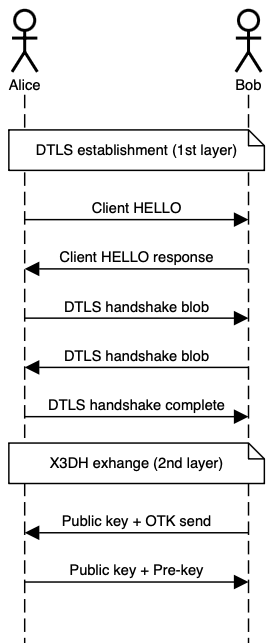
\includegraphics[scale=0.4]{./authentification/diagram.png}
    \caption{Diagram of exchanges before the the first message.}
\end{figure}

\section{Datagram Transport Layer Security}
\label{sec:dtls}

Datagram Transport Layer Security (DTLS) is a protocol based on TLS, designed 
to prevent eavesdropping, tampering, and message forgery \cite{rfc9147}. It 
guarantees a reliable and in-order delivery of data, unlike datagram transport. 
DLTS is the first security layer of the Turms protocol. You MUST implement a 
first security layer, ensuring encryption, authenticity and integrity.
\bigskip

See: \href{https://datatracker.ietf.org/doc/rfc9147/}{RFC 9147}.

\section{Extended Triple Diffie-Hellman}

In P2P, there is no trusted server to guarantee that Alice and Bob's public 
keys are correct. The security layer provided by DTLS ensures that the keys 
have not been altered by a third party (MITM).
\bigskip

If Alice initiated the WebRTC connection, then Bob initiates the key exchange. 
Bob, as initiator, send to Alice its public key and one-time key \((IK_B, 
OPK_B)\).

\begin{align*}
    DH_1 &= DH(IK_B, SPK_A)\\
    DH_2 &= DH(EK_B, IK_A)\\
    DH_3 &= DH(EK_B, SPK_A)\\
    DH_4 &= DH(EK_B, OPK_A)\\
    SK &= \mathrm{KDF}_{\text{Concat}}\left( DH_1 \,\|\, DH_2 \,\|\, DH_3 
\,\|\, DH_4 \right)
\end{align*}

with \(\mathrm{KDF}\) a key derivation function, often based on HKDF with 
SHA-256.

\begin{align*}
    (\text{RootKey}, \text{ChainKey}) &= \mathrm{KDF}_{\text{Root}}(SK)\\
    \text{MessageKey} &= \mathrm{KDF}_{\text{Chain}}(\text{ChainKey})
\end{align*}

Bob checks Alice's pre-signed \(SPK_A\) is authentic:

\begin{equation*}
    \mathrm{VerifySig}(IK_A, \mathrm{Sig}_{IK_A}(SPK_A)) = 1
\end{equation*}

As described on Signal's specification, \enquote{the parties may compare their 
identity public keys \(IK_A\) and \(IK_B\) through some authenticated 
channel}\cite[p. 7]{marlinspike2016}. Turms has chosen to ensure P2P security 
by conducting exchanges over the secure DTLS channel. You MUST implement DTLS 
connection before exchange public keys. This choice mitigate subsections 4.1, 
4.7 and 4.8 of X3DH protocol \enquote{Security 
considerations}\cite{marlinspike2016}, but creates possible non-deniability of 
communication between peers.

\section{Double Ratchet}

The Double Ratchet protocol extends X3DH by ensuring \enquote{Perfect Forward 
Secrecy} and \enquote{Post-Compromise Security}\cite{perrin2025}. It combines
two key update mechanisms:
\begin{itemize}
    \item one Diffie-Hellman key ratchet (asymmetric);
    \item un symmetrical ratchet (based on a KDF).
\end{itemize}

After the X3DH exchange, both parties have the same initial root key:

\[
    RK_0 = \text{KDF}_{\text{Root}}(SK_{\text{X3DH}})
\]

Each party also has a pair of initial Diffie-Hellman keys:

\[
    (DH_s^{(0)}, DH_r^{(0)})
\]

Each time a new public key \(DH_r^{(t)}\) is received from the other party:
\begin{align*}
    DH_{\text{out}}^{(t)} &= DH(DH_s^{(t-1)}, DH_r^{(t)}) \\
    RK_t, CK_r^{(t)} &= \mathrm{KDF}_{\text{Root}}(RK_{t-1}, 
DH_{\text{out}}^{(t)}) \\
    DH_s^{(t)} &\leftarrow \text{GenerateKeyPair()} \\
    RK_t, CK_s^{(t)} &= \mathrm{KDF}_{\text{Root}}(RK_t, DH(DH_s^{(t)}, 
DH_r^{(t)}))
\end{align*}

Thus, with each Diffie-Hellman jump, the root key and the two strings 
(send/receive) are renewed. For each message sent, the send string is derived:

\[
    CK_s^{(i+1)}, MK_s^{(i)} = \mathrm{KDF}_{\text{Chain}}(CK_s^{(i)})
\]

For each message received:

\[
    CK_r^{(j+1)}, MK_r^{(j)} = \mathrm{KDF}_{\text{Chain}}(CK_r^{(j)})
\]

\begin{align*}
    \mathrm{Encrypt}(MK_s^{(i)}, &\text{plaintext}) \to \text{ciphertext}\\
    \mathrm{Decrypt}(MK_r^{(j)}, &\text{ciphertext}) \to \text{plaintext}
\end{align*}

A message key MUST NEVER be reused, to ensure perfect confidentiality of old 
messages even in the event of future compromise.

\begin{align*}
    RK_0 &= \mathrm{KDF}_{\text{Root}}(SK_{\text{X3DH}}) \\[6pt]
    RK_t, CK_r^{(t)} &= \mathrm{KDF}_{\text{Root}}\big(RK_{t-1}, 
DH(DH_s^{(t-1)}, DH_r^{(t)})\big) \\[6pt]
    RK_t, CK_s^{(t)} &= \mathrm{KDF}_{\text{Root}}\big(RK_t, DH(DH_s^{(t)}, 
DH_r^{(t)})\big) \\[6pt]
    CK_{x}^{(i+1)}, MK_{x}^{(i)} &= \mathrm{KDF}_{\text{Chain}}(CK_{x}^{(i)}), 
\quad x \in \{s, r\}
\end{align*}

\begin{itemize}
    \item \textbf{Perfect Forward Secrecy}: compromising a future key does not 
        reveal previous messages.
    \item \textbf{Post-Compromise Security}: after a DH jump, the new keys 
        become secure again.
    \item \textbf{Unidirectional derivation}: no derived key can be traced back 
        to the root key.
\end{itemize}